\section{Fase 2 - SpecReason e Gestione del Contesto}
\label{sec:fase2}

La seconda fase dell'architettura \texttt{HybridRepair}, denominata \textbf{SpecReason}, costituisce il nucleo
cognitivo del sistema: le informazioni diagnostiche prodotte dal \texttt{FaultOracle} vengono trasformate in
conoscenza operativa, ossia una specifica di riparazione strutturata che guiderà il modello \texttt{GPT-4o} nella
Fase 3. Il nome riflette la duplice vocazione: \textit{Spec} per la produzione di una specifica rigorosa (la
\texttt{RepairSpec}), \textit{Reason} per il paradigma di ragionamento forzato con cui tale specifica è elicitata
dal modello.

SpecReason mira a risolvere due famiglie di fallimento tipiche dell'APR basato su LLM, già discusse in precedenza:
\begin{itemize}
    \item \textbf{L'allucinazione:} il modello genera codice sintatticamente plausibile ma invoca metodi o campi
    inesistenti nella libreria target.
    \item \textbf{La deriva semantica:} il modello interpreta il bug come un pattern di correzione familiare appreso
    nel pre-training, anziché come problema specifico dell'istanza, allontanandosi dalla logica richiesta.
\end{itemize}

Per mitigare queste criticità, SpecReason si avvale di due meccanismi complementari: l'\textbf{Ingredient Forge},
che raccoglie proattivamente il vocabolario reale delle API dal codice sorgente e lo inietta nel prompt, e il
paradigma \textbf{Chain-of-Thought} (\texttt{spec\_builder.py}), che costringe il modello a esplicitare un
ragionamento sul difetto prima di scriverne la correzione. Un terzo livello di salvaguardia, \textbf{SpecCritic}
(\texttt{spec\_critic.py}), implementa un ciclo di auto-critica in cui una seconda chiamata al modello valuta la
coerenza logica della specifica confrontandola con le prove empiriche (stack trace, test falliti). L'artefatto
finale è una \texttt{RepairSpec} validata, contesto privilegiato per la Fase 3 (\texttt{PatchAgent}).

\newpage
\subsection{Il Flusso Dati}
\label{subsec:flusso_dati}

Il flusso di dati della Fase 2 è orchestrato dal modulo \texttt{repair\_bug.py}, che coordina l'esecuzione
sequenziale dei sotto-componenti:

\begin{lstlisting}[language=Python]
# Frammento da repair_bug.py - orchestrazione della Fase 2

# Ingredient Forge
ingredients = collect_ingredients(fault_report)        
# SpecBuilder (CoT)
spec = build_spec(fault_report, ingredients, client=client) 
# SpecCritic
spec = validate_spec(spec, fault_report, client=client)      
\end{lstlisting}


\begin{figure}[htbp]
    \centering
    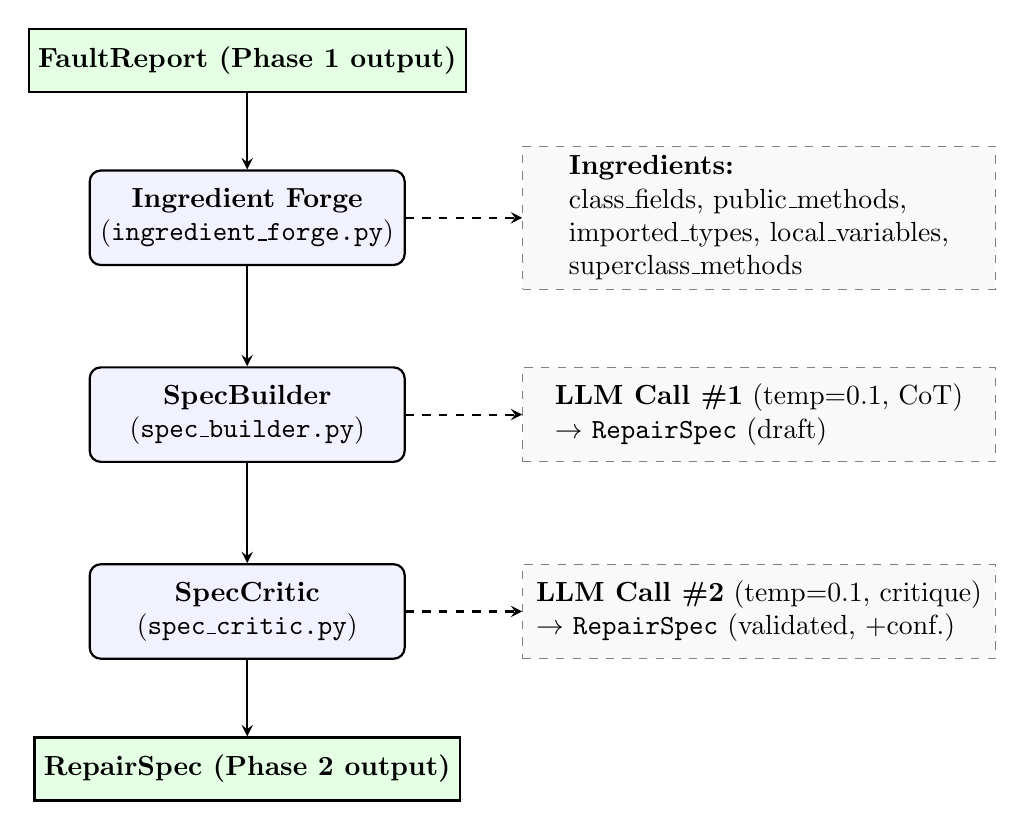
\begin{tikzpicture}[
        >=stealth,
        box/.style={rectangle, draw, thick, rounded corners, minimum width=4cm, minimum height=1.2cm, align=center, fill=blue!5},
        data/.style={rectangle, draw=gray, dashed, minimum width=6cm, minimum height=1.2cm, align=left, fill=gray!5},
        io/.style={rectangle, draw, thick, fill=green!10, text centered, minimum width=4cm, minimum height=0.8cm, font=\bfseries}
    ]

    % Blocchi principali
    \node[io]    (input)   at (0, 0) {FaultReport (Phase 1 output)};
    
    \node[box]   (forge)   at (0, -2) {\textbf{Ingredient Forge}\\(\texttt{ingredient\_forge.py})};
    \node[data]  (ingr)    at (6.5, -2) {\textbf{Ingredients:}\\class\_fields, public\_methods,\\imported\_types, local\_variables,\\superclass\_methods};
    
    \node[box]   (builder) at (0, -4.5) {\textbf{SpecBuilder}\\(\texttt{spec\_builder.py})};
    \node[data]  (llm1)    at (6.5, -4.5) {\textbf{LLM Call \#1} (temp=0.1, CoT)\\$\rightarrow$ \texttt{RepairSpec} (draft)};
    
    \node[box]   (critic)  at (0, -7) {\textbf{SpecCritic}\\(\texttt{spec\_critic.py})};
    \node[data]  (llm2)    at (6.5, -7) {\textbf{LLM Call \#2} (temp=0.1, critique)\\$\rightarrow$ \texttt{RepairSpec} (validated, +conf.)};
    
    \node[io]    (output)  at (0, -9) {RepairSpec (Phase 2 output)};

    % Collegamenti verticali
    \draw[->, thick] (input) -- (forge);
    \draw[->, thick] (forge) -- (builder);
    \draw[->, thick] (builder) -- (critic);
    \draw[->, thick] (critic) -- (output);
    
    % Collegamenti laterali
    \draw[->, thick, dashed] (forge) -- (ingr);
    \draw[->, thick, dashed] (builder) -- (llm1);
    \draw[->, thick, dashed] (critic) -- (llm2);

    \end{tikzpicture}
    \caption{Architettura e flusso dei dati della Fase 2.}
    \label{fig:schema_fase2}
\end{figure}


Il processo prende in input il \texttt{FaultReport} diagnostico. L'aspetto architetturale di maggior rilievo è
che le istruzioni fornite al modello sono costruite dinamicamente dal contesto, superando l'approccio dei prompt
statici. Questa composizione fonde due tipi di informazione: le catene causali semanticamente ancorate prodotte
da \texttt{LogicFL} (risolte tramite \texttt{prolog\_grounding.py}) e gli ``ingredienti'' statici estratti dal
codice sorgente da \texttt{ingredient\_forge.py}. Ogni prompt risulta così radicato nella specificità del bug
corrente, evitando che il modello si appoggi alla propria memoria parametrica, che in debugging potrebbe
suggerire pattern obsoleti o API inesistenti.

\subsection{Ingredient Forge: la Raccolta Proattiva del Contesto Statico}
\label{subsec:3_3_2}

L'allucinazione — la generazione di patch che invocano metodi o campi inesistenti nella libreria target —
scaturisce dal fatto che il modello, addestrato su milioni di frammenti Java eterogenei, apprende le distribuzioni
statistiche dei pattern di codifica ma non ha accesso all'interfaccia pubblica effettiva della classe da riparare.
Per neutralizzarla, il modulo \texttt{ingredient\_forge.py} implementa la \textit{context injection}: anziché
confidare nella memoria parametrica del modello, il vocabolario reale della classe viene estratto dal codice
sorgente difettoso e iniettato nel prompt come vincolo esplicito. L'approccio trae ispirazione da sistemi allo
stato dell'arte come \texttt{FitRepair} \cite{xia2024fitrepair} e \texttt{ReinFix} \cite{zhang2026reinfix}, che
hanno mostrato come la pre-iniezione di codice reale riduca le allucinazioni; \texttt{HybridRepair} ne sistematizza
l'idea estraendo molteplici categorie di ingredienti statici.

\subsubsection{Architettura del Modulo ingredient\_forge.py}
L'architettura di \texttt{ingredient\_forge.py} si impernia sulla funzione coordinatrice \texttt{collect()}, che
orchestra cinque funzioni private di analisi sintattica per produrre un oggetto \texttt{Ingredients}. La scelta
metodologica più rilevante è l'uso di espressioni regolari (regex) per il parsing del sorgente grezzo, scartando
i parser AST completi (Tree-sitter, JavaParser). La decisione è motivata da esigenze di robustezza: nell'APR il
codice in input è per definizione difettoso e un parser AST rigido fallirebbe in modo irrecuperabile su input
malformato, bloccando la pipeline. Le regex, invece, sono elastiche: ignorano il rumore di fondo ed estraggono
firme di metodi e variabili anche con sintassi compromessa. Sono compilate staticamente una sola volta per processo.

\begin{lstlisting}[language=Python]
# Estratto da ingredient_forge.py - compilazione statica dei pattern regex
_PUBLIC_METHOD_RE = re.compile(
    r"^\s*"
    r"(?:@\w+(?:\([^)]*\))?\s*)*"                     # optional annotations
    r"(public|protected)\s+"
    r"(?:static\s+|final\s+|abstract\s+|synchronized\s+|native\s+|strictfp\s+)*"
    r"(?:<[^>]+>\s+)?"                                # generic params
    r"([\w<>\[\],.\\s?]+?)\s+"                         # return type
    r"(\w+)\s*\(([^)]*)\)",                           # name(params)
    re.MULTILINE,
\end{lstlisting}

Prima di tentare qualsiasi estrazione, il modulo applica però una fondamentale fase
di pre-processing tramite la funzione \texttt{\_strip\_comments()}. Questa funzione rimuove
sia i commenti in blocco (\texttt{/* ... */}) sia i commenti
in linea (\texttt{// ...}) esplorando il testo con due passaggi
separati. Eliminare i commenti è un passo critico per
prevenire i falsi positivi: senza questa operazione preliminare, le
regex estrarrebbero erroneamente firme di metodi menzionate a scopo
documentale all'interno del \texttt{JavaDoc} o frammenti di codice ``commentato''
dagli sviluppatori.

Il cuore estrattivo del modulo è particolarmente evidente nella logica
ingegneristica che governa l'espressione regolare \texttt{\_PUBLIC\_METHOD\_RE}, deputata alla
cattura delle firme dei metodi. Anziché limitarsi a una
semplice ricerca di nomi e parentesi, la regex è
strutturata con gruppi di cattura sofisticati che riflettono precise
scelte di design:

Gestione delle annotazioni: Il codice di produzione Java è
tipicamente ricco di annotazioni. Un gruppo non catturante 
\texttt{((?:@\textbackslash{}w+(?:\textbackslash{}([\^{})]*\textbackslash{})\textbackslash{})?\textbackslash{}s*)*)}
è stato progettato per ignorare in modo elegante zero o
più annotazioni, come \texttt{@Override}, \texttt{@Nullable} o \texttt{@SuppressWarnings("unchecked")}. Se
la regex non gestisse queste strutture, la quasi totalità
dei metodi sovrascritti o annotati verrebbe semplicemente ignorata dall'estrattore.

Gestione flessibile dei modificatori: I modificatori di accesso e
di comportamento (static, final, abstract, synchronized, ecc.) sono resi
opzionali all'interno del pattern, permettendo al sistema di mappare
con successo ogni combinazione legale permessa dalla grammatica Java.

Supporto ai tipi generici: Un ulteriore gruppo dedicato \texttt{((?:<[\^{}>]+>\textbackslash{}s+)?)}
permettedi riconoscere e oltrepassare le dichiarazioni di tipi generici
a livello di metodo (es. \texttt{public <T extends Comparable<T>> T max(T a, T b)}).
Poiché le classi di utilità in dataset come \texttt{Defects4J}
fanno un uso massiccio dei generics, catturarli correttamente garantisce
che la firma estratta sia integra e fedele alla dichiarazione
originale.

\subsubsection{Le Categorie di Contesto Statico}
\label{subsubsec:3_3_2_3}
La funzione pubblica \texttt{collect()}, cuore del modulo, orchestra l'estrazione
di informazioni costruendo un oggetto popolato da cinque attributi distinti,
ciascuno dei quali rappresenta una specifica categoria di contesto statico.
L'estrazione mirata di queste cinque categorie è vitale per fornire
al modello linguistico una mappa completa e accurata dell'ambiente di
esecuzione, scongiurando errori di compilazione nella patch finale.
\begin{itemize}
\item \textbf{1. Campi della classe} Questa categoria raccoglie i campi di
istanza e statici della classe sotto esame. 

\begin{lstlisting}[language=Python]
# Estratto da _extract_fields() in ingredient_forge.py
_FIELD_RE = re.compile(
    r"^\s*(?:(?:public|protected|private|static|final|transient|volatile)\s+)*"
    r"([\w<>\[\],.?]+)\s+(\w+)\s*[;=]",
    re.MULTILINE,
\end{lstlisting}

Il pattern di estrazione è progettato per riconoscere le diverse combinazioni di visibilità
e di modificatori, separando il tipo e il nome
della variabile. \\Viene inoltre applicato un filtro rigoroso per escludere
eventuali falsi positivi derivanti da parole chiave del linguaggio Java
(come \texttt{class}, \texttt{interface} o \texttt{return}). L'inclusione di questi campi nel
prompt è cruciale: essa rivela al modello lo stato interno
attualmente disponibile all'interno della classe (ad esempio, le variabili d'istanza),
permettendogli di utilizzarlo per la risoluzione del bug senza dover
fare affidamento sulla propria memoria parametrica.
\item \textbf{2. Metodi pubblici della classe} Le firme complete dei metodi
pubblici, comprensive di modificatori di accesso, tipo di ritorno, nome
e parametri, vengono estratte sistematicamente. Il sistema è in grado
di catturare anche i costruttori pubblici e protetti, distinguendoli dai
metodi ordinari. 

\begin{lstlisting}[language=Python]
_PUBLIC_CONSTRUCTOR_RE = re.compile(
    r"^\s*"
    r"(?:@\w+(?:\([^)]*\))?\s*)*"
    r"(public|protected)\s+"
    r"(\w+)\s*\(([^)]*)\)\s*(?:throws [^{]+)?\s*\{",
    re.MULTILINE,
\end{lstlisting}

La gestione delle clausole \texttt{throws} consente di riconoscere le firme anche con eccezioni controllate; una
fase di deduplicazione evita che metodi ripetuti (es. in classi anonime) inquinino il prompt. Fornire questa
lista garantisce che il modello invochi solo metodi realmente esistenti e accessibili.
\item \textbf{3. Metodi della superclasse} \texttt{HybridRepair} risolve ed estrae anche i metodi ereditati. La
logica opera in due fasi: prima una regex cattura il nome della superclasse dalla dichiarazione \texttt{extends};

\begin{lstlisting}[language=Python]
_EXTENDS_RE = re.compile(
    r"\bextends\s+([\w.]+)",
)
\end{lstlisting}

poi il sistema ricerca ricorsivamente il file sorgente corrispondente nei source roots del progetto.

\begin{lstlisting}[language=Python]
# Estratto della seconda fase in _resolve_superclass_file()
simple = super_name.split(".")[-1] + ".java"
for root in source_roots:
    hits = list(root.rglob(simple))
    if hits:
        return hits[0] # Ritorna il file sorgente della superclasse
\end{lstlisting}


Questa categoria è importante soprattutto nei bug NULL\_RETURN legati all'override: rendere l'LLM consapevole che
un metodo sovrascrive un'implementazione genitrice lo guida verso patch più rispettose del contratto ereditato.

\item \textbf{4. Tipi importati} L'estrazione degli import assolve a due funzioni strategiche.

\begin{lstlisting}[language=Python]
_IMPORT_RE = re.compile(
    r"^\s*import\s+([\w.]+)\s*;",
    re.MULTILINE,
\end{lstlisting}

Da un lato espone il namespace esatto dei tipi utilizzabili nel file, evitando che il modello proponga classi non
importate; dall'altro segnala la versione delle dipendenze in uso (sapere se il file usa
\texttt{org.apache.commons.lang.StringUtils} o la variante \texttt{lang3} guida verso costrutti compatibili con
l'ambiente del bug).
\item \textbf{5. Variabili locali nel corpo del metodo difettoso} È la categoria a maggior specificità
contestuale: l'estrazione è limitata al corpo del metodo che contiene il difetto, analizzando le dichiarazioni
visibili in prossimità della riga di fault (incluso il modificatore \texttt{final}).

\begin{lstlisting}[language=Python]
# Estratto da _extract_local_variables() in ingredient_forge.py
var_re = re.compile(
    r"^\s*(?:final\s+)?([\w<>\[\],.?]+)\s+(\w+)\s*[;=]"
)
\end{lstlisting}


Questa informazione previene i conflitti di scoping: costringe il modello a riutilizzare variabili già
dichiarate e inizializzate, evitando re-inizializzazioni ridondanti o nuovi identificatori in collisione che
causerebbero errori di compilazione.
\end{itemize}
\subsubsection{La Struttura Dati Ingredients}
\label{subsubsec:3_3_2_4}
Il contratto di dati è formalizzato nella struttura \texttt{Ingredients}.

\begin{lstlisting}[language=Python]
@dataclass
class Ingredients:
    """Contesto statico raccolto proattivamente da IngredientForge.
    Iniettato nel prompt del LLM per evitare che allucini.
    """
    class_fields: List[str] = field(default_factory=list)
    """Dichiarazioni dei campi della classe target."""

    public_methods: List[str] = field(default_factory=list)
    """Firme dei metodi pubblici/protetti della classe target."""

    superclass_methods: List[str] = field(default_factory=list)
    """Metodi pubblici ereditati dalle superclassi dirette."""

    imported_types: List[str] = field(default_factory=list)
    """Tipi fully-qualified importati nel file sorgente."""

    local_variables: List[str] = field(default_factory=list)
    """Variabili visibili nello scope della riga di errore."""

    caller_context: str = ""
\end{lstlisting}

La struttura è volutamente ``piatta'' (liste di stringhe a un solo livello), in contrasto con AST o oggetti JSON
annidati. Le stringhe sono il formato nativo dei token su cui operano gli LLM: fornendole pre-formattate si
elimina una serializzazione costosa e soggetta a perdita di informazioni, massimizzando efficienza e
intelligibilità dell'input.
\newpage
\subsubsection{Il Meccanismo di Iniezione: dalla Struttura al Prompt}
\label{subsubsec:3_3_2_5}
L'ultimo passaggio inietta i dati raccolti nel prompt utente tramite la funzione helper \texttt{\_format\_list()}.

\begin{lstlisting}[language=Python]
def _format_list(items: list, max_items: int = 20) -> str:
    """Format a list as a comma-separated string, truncating if needed."""
    if not items:
        return "(none available)"
    truncated = items[:max_items]
    result = ", ".join(f"`{item}`" for item in truncated)
    if len(items) > max_items:
        result += f" ... (+{len(items) - max_items} more)"
\end{lstlisting}

Il meccanismo concentra tre decisioni di prompt engineering:
\begin{itemize}
    \item \textbf{Troncamento a 20 elementi} per lista, bilanciamento empirico tra completezza e \textit{context
    pressure}: iniettare centinaia di metodi saturerebbe la finestra di contesto, distogliendo l'attenzione del
    modello dalle informazioni diagnostiche primarie.
    \item \textbf{Backtick Markdown} attorno a ogni elemento come \textit{instruction reinforcement}: gli LLM
    associano i backtick a identificatori letterali e tendono a trattarli come entità intoccabili, riducendo il
    rischio di parafrasi o mutazioni sintattiche.
    \item \textbf{Fallback ``(none available)''} per le liste vuote: una stringa esplicita anziché uno spazio
    vuoto evita che il modello interpreti il campo come un errore di formattazione o un dato mancante.
\end{itemize}
Per un bug come \texttt{JacksonDatabind-3}, l'iniezione produce una sezione del prompt della forma:

\begin{verbatim}
### Available API (Repair Ingredients)
**Class fields:** 
`ObjectMapper _objectMapper`, `boolean _configured`, ...
**Public methods:** 
`public void setMapper(ObjectMapper mapper)`, ...
**Imported types:** 
`com.fasterxml.jackson.databind.ObjectMapper`, `java.util.List`, ...
\end{verbatim}
\enlargethispage{1\baselineskip}
Tramite questa iniezione, il prompt si ancora all'istanza concreta del bug, vincolando lo spazio decisionale del
modello alla realtà del codice sorgente.

\subsection{Il Paradigma Chain-of-Thought: \texttt{spec\_builder.py}}
Il modulo \texttt{spec\_builder.py} è l'infrastruttura di ragionamento della Fase 2. Dopo la raccolta del contesto
statico, il sistema deve tradurre le informazioni diagnostiche in un piano d'azione coerente, affidandosi al
paradigma Chain-of-Thought (CoT) per forzare la scomposizione analitica del problema.

\subsubsection{Fondamento Teorico del Chain-of-Thought Prompting}
\label{subsubsec:3_3_3_1}
Il Chain-of-Thought prompting, formalizzato da Wei et al. \cite{wei2022chain}, si basa su un'intuizione semplice:
istruire il modello a produrre una catena di ragionamento intermedio prima della risposta finale migliora la
qualità dell'output. La probabilità di generare un token corretto al passo $t$ aumenta se preceduto da un
ragionamento esplicitato nei token antecedenti \cite{wei2022chain}.

Nell'APR il paradigma è imprescindibile: chiedere a un LLM di generare direttamente una patch da un report di
errore equivale a forzare un problema ``multi-hop'' in un singolo salto cognitivo, fondendo quattro operazioni
(comprendere il difetto, dedurre il comportamento corretto, isolare la differenza minima, tradurla in sintassi
Java). Costretto a eseguirle in parallelo, il modello tende a scorciatoie cognitive — pattern di fix generici
come un null-check casuale — rinunciando a una soluzione mirata per l'istanza.

La validità del CoT nell'APR è dimostrata da sistemi come \texttt{ThinkRepair} \cite{yin2024thinkrepair}, dove
l'anteposizione di un passo di ragionamento (``think step by step'') incrementa il tasso di successo su
\texttt{Defects4J} di circa 15 punti percentuali. \texttt{HybridRepair} radicalizza l'approccio: anziché una
richiesta di ragionamento libera, costringe il modello a rispondere a tre interrogativi puntuali in formato XML
rigoroso, rendendo ogni fase parzialmente verificabile in modo automatico.


\newpage
\subsubsection{Architettura del System Prompt di SpecBuilder}
\label{subsubsec:3_3_3_2}
Il prompting di \texttt{spec\_builder.py} sfrutta l'architettura a messaggi dell'API OpenAI, separando un
\textit{system prompt} (che definisce la persona del modello e i suoi confini comportamentali) da uno \textit{user
prompt} (che inietta i dati dell'istanza). Il system prompt di \texttt{SpecBuilder} è il seguente:

\begin{lstlisting}[language=Python]
SPEC_SYSTEM_PROMPT = """\
You are an expert Java bug analyst. Your task is to reason about a bug \
BEFORE writing any code. You must provide a precise natural-language \
specification of the fix, NOT the code itself.

Respond ONLY in the structured format below no code, no diffs, no patches.\
"""
\end{lstlisting}

Pur composto da poche parole, il \texttt{SPEC\_SYSTEM\_PROMPT} concentra tecniche di \textit{instruction
reinforcement} \cite{white2023prompt}. Il maiuscolo su ``BEFORE'' (``reason about a bug BEFORE writing any code'')
spezza l'autocompletamento istintivo: essendo gli LLM autoregressivi, un contesto saturo di codice Java li induce
a generare subito altro codice \cite{brown2020language}, e imporre una precedenza temporale disinnesca questo
riflesso. I vincoli negativi (``NOT the code itself'', ``no code, no diffs, no patches'') esplicitano i divieti,
fondamentali per reprimere comportamenti eseguiti per inerzia generativa \cite{ouyang2022training}; il token
``ONLY'' funge da guardrail contro prosa libera e commenti che comprometterebbero il parsing XML deterministico
\cite{white2023prompt}.

\subsubsection{Il Template del Prompt Utente: Anatomia di \texttt{SPEC\_USER\_TEMPLATE}}
\label{subsubsec:3_3_3_3}
Se il system prompt stabilisce le regole d'ingaggio, il \texttt{SPEC\_USER\_TEMPLATE} costituisce
la mappa operativa in cui il modello deve navigare:

\begin{lstlisting}[language=Python]
SPEC_USER_TEMPLATE = """\
## Bug Analysis Task

**Bug ID:** {bug_id}

### Fault Location
- **Class:** `{class_name}`
- **Line:** {line}
- **Method:**
```java
{method_source}
```

### Prolog Causal Analysis (from LogicFL - Semantically Grounded)
{causal_analysis}

### Repair Directives (from Prolog Rule Analysis)
{repair_directives}

### Failing Test(s)
{failing_tests}

### Stack Trace
```
{stack_traces}
```

### Available API (Repair Ingredients)
**Class fields:** {class_fields}
**Public methods:** {public_methods}
**Imported types:** {imported_types}
**Local variables:** {local_variables}

---

## Your Task

Answer these three questions precisely and concisely:

### 1. Flawed Behavior
What does the buggy method currently do wrong? Be specific about the \
exact line and the nature of the defect (e.g., "line 42 dereferences \
`result` which can be null when the input array is empty").

### 2. Intended Behavior
What SHOULD the method do? Infer this from the test expectations and \
any JavaDoc comments. Be specific.

### 3. Minimal Fix
What is the SMALLEST conceptual change that fixes the bug? Describe it \
in plain English (e.g., "Add a null check for `result` before line 42, \
returning an empty array if null"). Do NOT write code.

Respond in this exact format:
<flawed_behavior>...</flawed_behavior>
<intended_behavior>...</intended_behavior>
<minimal_fix>...</minimal_fix>
\end{lstlisting}

Il template ha una struttura bipartita separata da un delimitatore orizzontale (\texttt{---}): un Blocco di
Evidenza e un Blocco di Compito.

\textbf{Il Blocco di Evidenza} aggrega le informazioni diagnostiche delle fasi precedenti: Bug ID e Fault
Location col sorgente del metodo, la Prolog Causal Analysis e le Repair Directives generate da \texttt{LogicFL},
e le tracce empiriche del fallimento (Failing Tests e Stack Trace). In chiusura, la sezione ``Available API
(Repair Ingredients)'' incorpora campi, metodi pubblici, tipi importati e variabili locali estratti
dall'Ingredient Forge. Il loro posizionamento in fondo al blocco non è casuale: collocare le API reali subito
prima del Task sfrutta il \textit{recency bias} dei Transformer \cite{zhao2021calibrate}, mitigando l'effetto
\textit{Lost in the Middle} \cite{liu2024lost} e riducendo il rischio che l'attenzione divaghi verso librerie allucinate.

\textbf{Il Blocco di Compito}, oltre il separatore, chiede al modello di rispondere a tre domande specifiche:
\begin{itemize}
    \item \textit{Flawed Behavior}: cosa fa di sbagliato il metodo, con la riga esatta;
    \item \textit{Intended Behavior}: cosa dovrebbe fare, inferendolo dalle aspettative dei test o dai JavaDoc;
    \item \textit{Minimal Fix}: la più piccola alterazione logica che risolve il problema, in linguaggio naturale
    e senza scrivere codice.
\end{itemize}
La separazione tramite delimitatori impedisce la sovrapposizione tra contesto e istruzioni \cite{white2023prompt};
l'incapsulamento della risposta in tag pseudo-XML (\texttt{<flawed\_behavior>}, ecc.) applica il \textit{format
manager pattern} \cite{white2023prompt}, essenziale per il parsing deterministico a valle.

\subsubsection{La Costruzione Dinamica del Prompt: \_build\_spec\_prompt()}
\label{subsubsec:3_3_3_4}
Una volta definiti i template statici e raccolti tutti
gli ingredienti necessari, il sistema deve fondere queste eterogenee
fonti di informazione in un unico prompt testuale coerente.
Questa delicata operazione di assemblaggio è demandata alla funzione
interna \texttt{\_build\_spec\_prompt()}.

\begin{lstlisting}[language=Python]
def _build_spec_prompt(
    fault_report: FaultReport,
    ingredients: Ingredients,
) -> str:
    primary = fault_report.locations[0] if fault_report.locations else None

    if fault_report.grounded_chains:
        from fault_oracle.prolog_grounding import format_grounded_chains
        causal_analysis = format_grounded_chains(fault_report.grounded_chains)
        directives = []
        for gc in fault_report.grounded_chains:
            if gc.repair_directive:
                directives.append(f"- {gc.repair_directive}")
        repair_directives = "\n".join(directives) if directives else "(none)"
    else:
        causal_analysis = "\n".join(fault_report.causal_chains) or "(none)"
        repair_directives = "(no rule-based directives available)"

    return SPEC_USER_TEMPLATE.format(
        bug_id=fault_report.bug_id,
        class_name=primary.class_name if primary else "unknown",
        line=primary.line if primary else 0,
        method_source=primary.method_source if primary else "(not available)",
        causal_analysis=causal_analysis,
        repair_directives=repair_directives,
        failing_tests="\n".join(
            f"- `{t['class']}::{t.get('method', '?')}`"
            for t in fault_report.failing_tests
        ) or "(none)",
        stack_traces=fault_report.stack_traces[:3000] or "(none)",
        class_fields=_format_list(ingredients.class_fields),
        public_methods=_format_list(ingredients.public_methods),
        imported_types=_format_list(ingredients.imported_types),
        local_variables=_format_list(ingredients.local_variables),
\end{lstlisting}

La funzione non è una semplice interpolazione di stringhe: incarna il principio della \textit{graceful
degradation}. Le catene causali di \texttt{LogicFL} sono idealmente arricchite dalla pipeline di Semantic
Grounding, ma l'analisi statica può fallire (sorgente non localizzabile, Tree-sitter in errore su sintassi
malformata, output LogicFL imprevisto). Anziché bloccare la pipeline, la funzione ripiega automaticamente sulle
catene causali Prolog grezze: il prompt risulta meno ricco, ma l'esecuzione prosegue fornendo comunque all'LLM
una traccia logica essenziale.

Completato l'assemblaggio, \texttt{SpecBuilder} invoca il modello tramite il client Azure OpenAI con temperatura
molto bassa (\texttt{temperature=0.1}). A differenza dei task creativi, dove valori prossimi a 1.0 massimizzano
la diversità \cite{sun2024exploring}, nel ragionamento deduttivo la variabilità è controproducente: il sistema
cerca la spiegazione fattualmente più probabile dalle prove empiriche. Una temperatura di 0.1 riduce la varianza
del campionamento, massimizza l'aderenza ai fatti, mitiga le allucinazioni \cite{kabakus2026evaluating} e
garantisce la riproducibilità della specifica.

\subsubsection{Il Parsing XML della Risposta e la Struttura RepairSpec}
\label{subsubsec:3_3_3_5}
La risposta del modello deve essere decodificata in una struttura dati. Il sistema impone l'incapsulamento delle
deduzioni in un formato XML semi-strutturato con tre tag (\texttt{<flawed\_behavior>}, \texttt{<intended\_behavior>},
\texttt{<minimal\_fix>}). La scelta dell'XML rispetto al JSON è motivata dalla robustezza: la grammatica JSON è
severa (escape delle virgolette, newline non ammessi nelle stringhe) e forzare un LLM a produrre JSON valido con
testo libero multiparagrafo comporta un rischio elevato di errori di parsing \cite{structuredrag2024}. L'XML, al
contrario, tollera nativamente testo discorsivo e ritorni a capo \cite{XMLPrompting2026}, ed è ampiamente
rappresentato nel corpus di pre-training (HTML, file di configurazione), risultando più affidabile.
Per estrarre il contenuto dei tag, \texttt{spec\_builder.py} implementa un parser a espressioni regolari.

La funzione interna di parsing, \texttt{\_parse\_spec\_response()}, si avvale di una regex meticolosamente
progettata: \texttt{rf"<\{tag\}>\textbackslash{}s*(.*?)\textbackslash{}s*</\{tag\}>"} accoppiata al flag di compilazione \texttt{re.DOTALL}.

\begin{lstlisting}[language=Python]
def _parse_spec_response(response: str) -> RepairSpec:
    import re

    def extract(tag: str) -> str:
        m = re.search(rf"<{tag}>\s*(.*?)\s*</{tag}>", response, re.DOTALL)
        return m.group(1).strip() if m else ""

    return RepairSpec(
        flawed_behavior=extract("flawed_behavior"),
        intended_behavior=extract("intended_behavior"),
        minimal_fix=extract("minimal_fix"),
\end{lstlisting}

L'ingegneria di questa espressione regolare garantisce la massima tolleranza
alle imprefezioni stilistiche del modello:
Il flag \texttt{re.DOTALL} è vitale poiché istruisce il metacarattere punto
(.) a riconoscere anche i caratteri di newline (\textbackslash{}n),
permettendo la cattura di testi distribuiti su più righe.
I gruppi \textbackslash{}s* posizionati subito dopo il tag di apertura
e subito prima del tag di chiusura assorbono in
modo flessibile eventuali spaziature o ritorni a capo spuri
introdotto dal modello, garantendo che il blocco di testo
utile venga catturato in modo pulito.
Il cuore della regex è il gruppo di cattura
\texttt{(.*?)}, che utilizza il quantificatore lazy \texttt{?}. In
assenza di questo quantificatore, l'operatore \texttt{.*} si comporterebbe in
modo ``ingordo'', consumando tutto il testo fino all'ultimo tag
di chiusura incontrato nell'intera stringa. Se il modello dovesse
inavvertitamente generare tag duplicati, un quantificatore avido distruggerebbe la
frammentazione logica della risposta. Il quantificatore lazy, al contrario,
garantisce che l'estrazione si fermi esattamente al primo tag
di chiusura corrispondente, garantendo una cattura robusta e sicura.
Un'ultima chiamata al metodo \texttt{.strip()} rimuove eventuali spaziature marginali
residue, restituendo il testo puro.
Il risultato di questo processo di estrazione viene infine
incapsulato all'interno della struttura \texttt{RepairSpec}.

\begin{lstlisting}[language=Python]
@dataclass
class RepairSpec:
    """Natural-language specification produced by Phase 2 (SpecReason).
    The LLM reasons about the bug *before* generating any code.
    """
    flawed_behavior: str = ""
    """What the buggy method currently does wrong."""

    intended_behavior: str = ""
    """What the method *should* do, inferred from tests + JavaDoc."""

    minimal_fix: str = ""
    """Conceptual description of the smallest change that fixes the bug."""

\end{lstlisting}

La \texttt{RepairSpec} è un oggetto immutabile, artefatto di trasferimento verso le fasi successive. Mantenere i
tre campi in linguaggio naturale anziché in linguaggi di specifica formale (Alloy, JML) è strategico: il
linguaggio naturale è il medium ottimale per comunicare l'intento di correzione al \texttt{PatchAgent} della Fase 3.
A titolo esemplificativo, per un bug come Chart-4 (NPE da dereferenziazione di un renderer non verificato), la
\texttt{RepairSpec} parsata assume una forma analoga alla seguente:

\begin{lstlisting}

  "flawed_behavior": "The method getRenderer(int index) at line 1749 calls
    this.renderers.get(index), which can return null when no renderer has been
    set for the given index. The returned value is cast to XYItemRenderer and
    immediately stored in `r`, which is then dereferenced at line 4493 without
    a null check.",

  "intended_behavior": "The method should return a non-null XYItemRenderer for
    any valid index, falling back to the default renderer if no specific renderer
    has been assigned to that index. The test expects that getRenderer(0) returns
    the default renderer when the list at index 0 is null or empty.",

  "minimal_fix": "After the cast on line 1749, add a null check: if `r` is null,
    return the default renderer (obtainable via getBaseRenderer() or by iterating
    the renderers list to find the first non-null entry).",

\end{lstlisting}

Questo artefatto cristallizza la comprensione del problema, trasformando dati di debug grezzi in un piano di
riparazione leggibile e pronto per essere tradotto in codice.

\subsection{SpecCritic: Validazione Autonoma della Specifica di Riparazione}
\label{subsec:3_3_4}
A valle di \texttt{SpecBuilder}, il modulo \texttt{spec\_critic.py} valuta, critica ed eventualmente emenda le
deduzioni della fase precedente.
\subsubsection{Il Problema della Coerenza Interna nelle Specifiche Generate da LLM}
\label{subsubsec:3_3_4_1}

Una \texttt{RepairSpec} generata in CoT può essere internamente coerente e plausibile ma fattualmente incongruente
con le prove empiriche \cite{cot_hallucinations_2025, dhuliawala2023chain}. Ad esempio, il modello potrebbe
identificare correttamente che \texttt{r} è \texttt{null} ma attribuirne l'origine a un metodo errato (confondendo
firme simili), oppure diagnosticare correttamente il difetto ma proporre una soluzione sovra-ingegnerizzata
(refactoring strutturale anziché un singolo controllo condizionale). Per arginare queste derive,
\texttt{spec\_critic.py} implementa un meccanismo di auto-critica ispirato alla Constitutional AI
\cite{bai2022constitutional}, qui declinato in forma alleggerita: un singolo turno di validazione mirato a
intercettare gli errori logici o fattuali più evidenti prima della generazione del codice.

\subsubsection{Il System Prompt del SpecCritic e la Separation of Concerns}
\label{subsubsec:3_3_4_2}
L'auto-critica si fonda sul principio della \textit{separation of concerns} traslato nel prompt engineering: se
lo \texttt{SpecBuilder} istruiva il modello come ``analista'', il system prompt dello SpecCritic gli impone il
ruolo opposto di ``meticulous code review expert'', incaricato di convalidare o rigettare il lavoro altrui.

\begin{lstlisting}[language=Python]
CRITIC_SYSTEM_PROMPT = """\
You are a meticulous code review expert. Your job is to validate a bug \
analysis produced by another analyst. Check for logical consistency, \
\end{lstlisting}

L'aspetto più sofisticato è il distanziamento psicologico: al modello si chiede di valutare un'analisi
``prodotta da un altro analista'' (\texttt{produced by another analyst}). Non è una finzione narrativa, ma una
contromisura tecnica contro la \textit{sycophancy} \cite{sharma2023sycophancy} e il \textit{self-enhancement
bias} \cite{zheng2023judging}: i modelli faticano ad auto-correggersi \cite{huang2024large} e tendono a validare
acriticamente i propri output se ne sono consapevoli autori. Fingendo una terza parte, si abbassa la barriera
difensiva del modello, incoraggiando una revisione severa e oggettiva.
\subsubsection{Il Template del Prompt del SpecCritic (CRITIC\_USER\_TEMPLATE)}
\label{subsubsec:3_3_4_3}
Il passaggio dal ruolo di generatore a quello di revisore
si riflette anche nell'architettura del prompt utente, il \texttt{CRITIC\_USER\_TEMPLATE}, che
presenta differenze strutturali e logiche profonde rispetto alla sua controparte
nello \texttt{SpecBuilder}.

\begin{lstlisting}[language=Python]
CRITIC_USER_TEMPLATE = """\
## Validation Task

An analyst produced the following bug specification. Validate it.

**Bug ID:** {bug_id}

### Analyst's Analysis

**Flawed Behavior:**
{flawed_behavior}

**Intended Behavior:**
{intended_behavior}

**Minimal Fix:**
{minimal_fix}

### Ground Truth (from test execution)

**Stack Trace:**
```
{stack_traces}
```

**Failing Tests:**
{failing_tests}

---

## Your Task

1. Is the "Flawed Behavior" description consistent with the stack trace?
2. Is the "Intended Behavior" plausible given the test expectations?
3. Is the "Minimal Fix" truly minimal, or does it over-engineer the solution?
4. Rate your confidence that this specification would lead to a correct fix (0.0-1.0).

If the analysis is correct, respond with the SAME content.
If corrections are needed, provide the corrected version.

Respond in this exact format:
<flawed_behavior>...</flawed_behavior>
<intended_behavior>...</intended_behavior>
<minimal_fix>...</minimal_fix>
<confidence>0.X</confidence>
"""
```
\end{lstlisting}


Il primo elemento di rottura è la sezione ``Ground Truth'', che raggruppa stack trace e test falliti
dall'esecuzione dinamica: la designazione segnala al modello che sono fatti empirici incontrovertibili, da far
prevalere sulle inferenze testuali in caso di conflitto. A seguire, il template sostituisce le domande aperte con
quattro criteri di validazione numerati che impediscono un'approvazione superficiale:
\begin{enumerate}
    \item \textbf{Coerenza logica}: la descrizione del difetto è coerente con la ``Ground Truth''?
    \item \textbf{Plausibilità fattuale}: l'intento correttivo è supportato dalle aspettative dei test?
    \item \textbf{Minimalità}: la correzione è genuinamente minimale o scade nell'over-engineering? Criterio
    critico nell'APR, dove le soluzioni invasive comportano un alto rischio di regressioni.
    \item \textbf{Confidence Score}: un giudizio quantitativo sulla robustezza della specifica.
\end{enumerate}
Infine, un'istruzione condizionale governa l'output: se la specifica è corretta, il modello restituisce l'XML
identico; se individua falle, genera direttamente l'XML emendato. Questa biforcazione evita parafrasi stilistiche
inutili e rende la critica immediatamente azionabile, arricchita dal quarto tag \texttt{<confidence>}, un float in
[0.0, 1.0] che quantifica la fiducia del critico nel fix.

\subsubsection{Il Parsing della Risposta e il Meccanismo di Fallback}
\label{subsubsec:3_3_4_4}
La trasformazione dell'output testuale del revisore in dati strutturati e
azionabili è affidata alla funzione interna \texttt{\_parse\_critic\_response()}.

\begin{lstlisting}[language=Python]
def _parse_critic_response(response: str) -> tuple[RepairSpec, float]:
    import re

    def extract(tag: str) -> str:
        m = re.search(rf"<{tag}>\s*(.*?)\s*</{tag}>", response, re.DOTALL)
        return m.group(1).strip() if m else ""

    confidence_str = extract("confidence")
    try:
        confidence = float(confidence_str)
    except (ValueError, TypeError):
        confidence = 0.5  # default if parsing fails

    return RepairSpec(
        flawed_behavior=extract("flawed_behavior"),
        intended_behavior=extract("intended_behavior"),
        minimal_fix=extract("minimal_fix"),
        confidence=confidence,
\end{lstlisting}

Da un punto di vista architetturale, questa funzione non si discosta dalla logica
basata su espressioni regolari già impiegata nello \texttt{SpecBuilder}, ma la
estende significativamente per accogliere l'estrazione del nuovo tag \texttt{<confidence>}. L'introduzione
Il parsing del nuovo tag \texttt{<confidence>} richiede un float in [0.0, 1.0] e una gestione rigorosa: il modello
potrebbe omettere il tag, inserirvi testo discorsivo (es. \texttt{<confidence>High (0.9)</confidence>}) o restituire
formati non convertibili. Di fronte a un \texttt{ValueError}/\texttt{TypeError} nel casting, la funzione adotta un
fallback conservativo a 0.5. Il valore mediano è calibrato: 0.0 penalizzerebbe ingiustamente una specifica magari
ineccepibile per un mero errore di formato, 1.0 le attribuirebbe un'affidabilità non verificata. Lo 0.5 segnala
un'incertezza formale dovuta a un intoppo tecnico; la funzione coordinatrice emette inoltre un log
(``\texttt{WARNING:} low confidence'') quando il valore scende sotto soglia.

La robustezza è ulteriormente garantita dalla funzione \texttt{validate()}: se l'LLM restituisce tag essenziali
(\texttt{<flawed\_behavior>}, \texttt{<minimal\_fix>}) vuoti o malformati, anziché scartare l'artefatto o inoltrare
un oggetto vuoto, il sistema recupera i campi originari dello \texttt{SpecBuilder} e li innesta al posto di quelli
vuoti. Nell'APR un contesto parziale vale più di un contesto assente: conservare il ragionamento originale evita
che il fallimento di un singolo controllo paralizzi l'intera pipeline.
\subsubsection{Il Flusso di Correzione Iterativa}
\label{subsubsec:3_3_4_5}
A differenza della Constitutional AI completa, che prevede cicli multi-iterativi fino a convergenza,
\texttt{HybridRepair} implementa un'auto-critica a singola iterazione. La scelta deriva da vincoli ingegneristici:
ogni chiamata a \texttt{GPT-4o} introduce latenza (2--10 s) e costo per token, e cicli a tre o più iterazioni
aggraverebbero i tempi della Fase 2 con un ROI computazionale sfavorevole \cite{chen2023frugalgpt}; in assenza di
feedback esterni, le iterazioni successive alla prima non garantiscono un miglioramento proporzionale al costo
\cite{valmeekam2023can}. Operativamente, una singola iterazione è sufficiente a intercettare le classi di errore
più comuni (inconsistenze con lo stack trace, over-engineering, errata localizzazione). Difetti più profondi (es.
semantiche di concorrenza) richiederebbero validazione formale o oracoli esterni \cite{shinn2023reflexion}, fuori
dalla portata di ulteriori iterazioni introspettive del medesimo modello.

\subsection{Integrazione nella Pipeline: il Contratto tra Fase 2 e Fase 3}
\label{subsec:3_3_5}
La Fase 2 si conclude producendo un oggetto \texttt{RepairSpec} validato, accompagnato dal set di
\texttt{Ingredients} raccolto. La transizione verso la generazione del codice è governata dall'orchestratore
\texttt{repair\_bug.py}, nel momento in cui viene istanziato il \texttt{PatchAgent}, motore della Fase 3.

\begin{lstlisting}[language=Python]
# Frammento da repair_bug.py - transizione Fase 2 -> Fase 3
agent = PatchAgent(
    fault_report=fault_report,
    repair_spec=spec,          # <- RepairSpec validata dalla Fase 2
    ingredients=ingredients,   # <- Ingredients raccolti dall'Ingredient Forge
    client=client,
)
\end{lstlisting}

Il costruttore riceve una triade di oggetti tipizzati: il \texttt{FaultReport} (eredità diagnostica della Fase 1),
la \texttt{RepairSpec} validata e gli \texttt{Ingredients} statici. Questa firma definisce un contratto software tra
i due macro-moduli, separando nettamente la strategia dagli strumenti: la \texttt{RepairSpec} descrive in linguaggio
naturale \emph{cosa} fare (comportamento difettoso, intento corretto, Minimal Fix) senza vincolarsi a implementazioni
premature, mentre gli \texttt{Ingredients} descrivono \emph{con quali strumenti} operare, fornendo l'inventario delle
API reali (campi, metodi, variabili locali, dipendenze). Il \texttt{PatchAgent} riceve così un duplice binario di
guida — direzione semantica dalla \texttt{RepairSpec} e contenimento sintattico dagli \texttt{Ingredients} —
trasformandosi da decisore incerto a esecutore vincolato.

L'interfaccia espone inoltre il valore \texttt{spec.confidence} calcolato durante l'auto-critica. Attualmente è reso
visibile nell'output diagnostico (log ``\texttt{RepairSpec} ready (confidence: X.XX)''); in evoluzioni future potrebbe
modulare la Fase 3, ad esempio aumentando il budget di campionamento per specifiche a bassa confidenza
(\texttt{confidence < 0.3}) o attivando modalità di repair differenziate (più conservative quando la fiducia è bassa).

